\chapter{Developer Notes}
\label{chap:dev}
In this chapter, we provide additional information for developers. 
\begin{figure}[t]
  \centering
  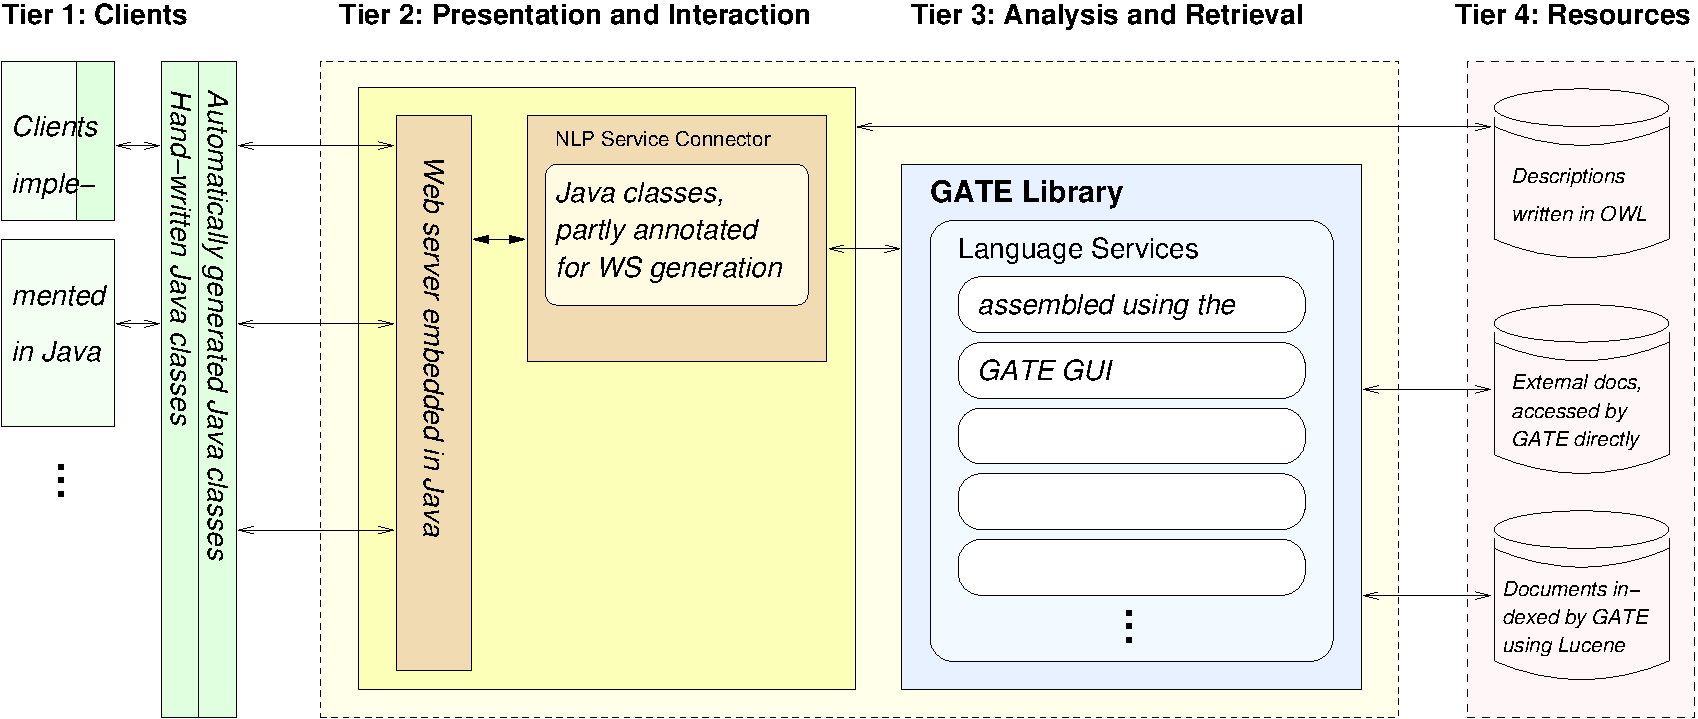
\includegraphics[width=\textwidth]{pictures/arch_impl}
  \caption{The architectural overview with implementation notes}
  \label{fig:arch_impl}
  \vspace*{-0.4cm}
\end{figure}

\section{Generic Compilation Instructions}
All parts of the \sa architecture (server, CSAL, clients) come with
ant build scripts that allow compilation from the command line
(usually \texttt{ant compile} or \texttt{ant run}).

\section{NetBeans Development}
The project has been developed using the NetBeans
IDE.\footnote{NetBeans IDE, \url{http://netbeans.org/}.} Debugging is
  made possible for all elements of the project, the steps will be
  described in this section. \textbf{Note:} The following steps have
  been validated with NetBeans IDE 6.7.

\subsection{Open the Project Workspace}

\begin{enumerate}
  \item Open the NetBeans IDE.
  \item Select \emph{File} from the Menu Bar then \emph{Open Project}.
  \item From the Dialog that pops-up navigate to the \emph{SemanticAssistants} Directory and open \emph{Server} and \emph{CSAL}. 
  \item Repeat the previous step and navigate to the \emph{SemanticAssistants/Clients} Directory and open \emph{OpenOffice} and \emph{CommandLine} 
\end{enumerate}

\subsection{Run a Project through NetBeans}

\begin{enumerate}
  \item Open the \emph{Files} Window (\emph{Ctrl-2}) and the list of the open project will appear.
  \item Collapse the files for a given project
  \item To \emph{compile/dist/run/clean} or any other action, \emph{R-Click} to the \emph{build.xml}, select \emph{Run target} and select one of the list.
\end{enumerate}

\subsection{Debug a Project with the NetBeans debugger}
\label{sec:debug}
Currently the projects: \emph{Server}, \emph{CSAL} and \emph{OpenOffice} are
being built with debug info and the developer has to follow the following
steps to attach the debugger in order to set breakpoints and pause the
execution of any given projects.  \textbf{Note:} To configure OpenOffice Writer
  to listen for incoming debugger connections please refer to the subsection 
  \emph{Configure the OpenOffice Writer to Run in Debug Mode} below.

\begin{enumerate}
  \item To debug a running process in the system, the developer should go to \emph{Debug} from the Menu bar and select \emph{Attach Debugger}. A window will pop up.
  \item Set the following arguments to the pop-up window: 
  \begin{itemize}
    \item \textbf{Debugger}: Java Debugger (JPDA)
    \item \textbf{Connector}: Socket Attach (Attaches by socket to other VMs)
    \item \textbf{Trasport}: dt\_socket 
    \item \textbf{Host:} The local machine's IP, e.g. \emph{Host: localhost}
    \item \textbf{Port:} The port that the process is listening. The value is found and changed at the build.xml. The \emph{Server} is listening at \emph{8888}.
  \end{itemize}
  \item Click \emph{OK}. The process that the debugger was attached, now runs in \emph{Debug Mode}.
	Repeat the above steps every time you run the project.
\end{enumerate}
  

\subsubsection{Configure the OpenOffice Writer to Run in Debug Mode}
This Section describes how to configure the JAVA VM in OpenOffice Writer to accept incoming connection for a debugger.

\begin{enumerate}
  \item Open OpenOffice Writer
  \item Go to Tools, Options. Under \emph{OpenOffice.org}, there is a \emph{Java} item. Select it and then Click on the 
        \emph{Parameter} button. There the parameters when running the JAVA VM are set.
  \item To run in debug mode \emph{Assign} the following 2 parameters:
  \begin{itemize}
    \item \textbf{-X debug}
    \item \textbf{-Xrunjdwp:transport=dt\_socket,server=y,suspend=n,address=7081}
  \end{itemize}
  \item \textbf{Note: The} \emph{address=7081} \textbf{should be the consistent with the port set in \emph{Attach Debugger} within NetBeans}
  \item  Now OO Writer is ready to accept connections from the debugger

\end{enumerate} 


\section{Service Descriptions}\label{sec:owl}
NLP services are described with metadata in OWL format. The ontology
format provides for expressive service description that captures
users, their language capabilities, tools, services, and result
formats. This allows connected clients to \emph{recommend} services
that are suitable for the current user, task, and output capabilities
(e.g., a cell phone has quite different output capabilities from a
netbook or desktop system). 


\subsection{Context and Service Representations}
\label{sec:contextservice}
Clients can request a list of available language services from the
server. Rather than simply returning all available services (which
could be a long list), we want to be able to \emph{recommend} possibly
useful NLP services to the user, based on her context.  In other
words, services that of no use are omitted, e.g., because of language
reasons or missing capabilities of the currently used client.  As a
first, minimal representation of the user's context, we enable a
client to communicate the languages that its user knows, as well as
the language of the document or documents in question. This
representation is recorded in Table~\ref{tab:context}.

\begin{table}[htb]
 \centering\small\sffamily
 \begin{tabular}{p{0.25\textwidth}@{\hspace*{4mm}}p{0.45\textwidth}@{\hspace*{4mm}}p{0.15\textwidth}}
 \toprule
 \textbf{Field} & \textbf{Meaning} & \textbf{Example} \\
 \midrule
 User languages& The languages the user knows& $<$en,de,fr$>$ \\
 Document language&The language of the current document &en \\
 \bottomrule
\end{tabular}
 \caption{Minimal representation of the user context}
 \label{tab:context}
\end{table}

For the client, the point of requesting a list of available language
services is to know which language services exist, and how it can
invoke them. Thus, each description sent by the server contains the
name of the language service it represents, so that the client can
identify it. Secondly, services might contain user-configurable
parameters, so the returned service description also contain a list of
parameter representations. Finally, for practical reasons, the
description holds a short, plain text description to make it clearer
what the language service achieves (examples can be seen in
Figure~\ref{fig:oolist}). Together, this gives us the NLP service
representations shown in Table~\ref{tab:service}

\begin{table}[htb]
 \centering\small\sffamily
 \begin{tabular}{p{0.15\textwidth}@{\hspace*{4mm}}p{0.40\textwidth}@{\hspace*{4mm}}p{0.3\textwidth}}
   \toprule
   \textbf{Field} & \textbf{Meaning} & \textbf{Example} \\
   \midrule
   Service & The name of the language & \emph{Single-document}\\ 
   name & service & \emph{summarizer} \\ 

   & & \\

   Service & Short description of what the & \emph{Creates a summary
     of} \\
   description & service achieves  & \emph{a single document} \\

   & & \\

   Parameter list & List of descriptions illustrated in
   Table~\ref{tab:param} & See Table~\ref{tab:param} \\
   \bottomrule
\end{tabular}
 \caption{Representation of an NLP service}
 \label{tab:service}
\end{table}


While service name and service description are simple strings, the
parameter list needs further clarification. This parameter
representation holds the parameter's name, its data type, and the
information whether the parameter is mandatory or
optional. Table~\ref{tab:param} shows its data fields in detail. In
addition to the mentioned fields, we added a \emph{Parameter value}
field to be written by the client, which it can use to announce
parameter values for a subsequent NLP service invocation. To increase
the usability, we added a \emph{Label} and a \emph{Description} field
that allows a system integrator to add some explaining words to the
parameter representation that are, e.g., helpful for user interface
integration.  The same holds for the \emph{Default Value} field, which
can be used to give the user an idea of what sensible parameter values
are.

% There is one more requirement related to the control of language
% services, and thus parameters. This requirement is Requirement~\#7.3,
% concerning the correct assignment of values.

\begin{table}[htb]
 \centering\small\sffamily
 \begin{tabular}{p{0.2\textwidth}@{\hspace*{4mm}}p{0.50\textwidth}@{\hspace*{4mm}}p{0.2\textwidth}}
   \toprule
   \textbf{Field} & \textbf{Meaning} & \textbf{Example} \\
   \midrule
   Parameter name & The (codified) name of the parameter &
   \emph{outputFormat} \\

   & & \\

   Parameter type & The data type of the parameter & \emph{string} \\

   & & \\

   Optional & Is the parameter optional or mandatory?  & \emph{no} \\

   & & \\

   Parameter value & The value the parameter should take for the
   following invocation. Field to be written by the client. &
   \emph{mediawiki} \\

   & & \\

   Parameter & A short description of the meaning of the & \emph{Use ``mediawiki''} \\
   description & parameter, or advice on its usage & \emph{ or ``html''} \\

   & & \\

   Label & A more expressive name suitable for display in user
   interfaces & \emph{Output format} \\

   & & \\

   Default value & A suitable standard value for the parameter & \emph{html} \\

   \bottomrule
\end{tabular}
 \caption{Representation of a parameter for an NLP service}
 \label{tab:param}
\end{table}

\subsection{The \sa Ontology}
In this section, we provide details on the design of the ontology
used for NLP service descriptions in the \sa architecture.

\subsubsection{The \sa Upper Ontology}
The \sa upper ontology contains five core concepts to model the
relationships between users, their tasks, the artifacts involved and
their format and language. Figure~\ref{fig:centralFive} shows these
five concepts and Table~\ref{tab:top5} provides some descriptions and
examples.

\begin{figure}
  \centering
  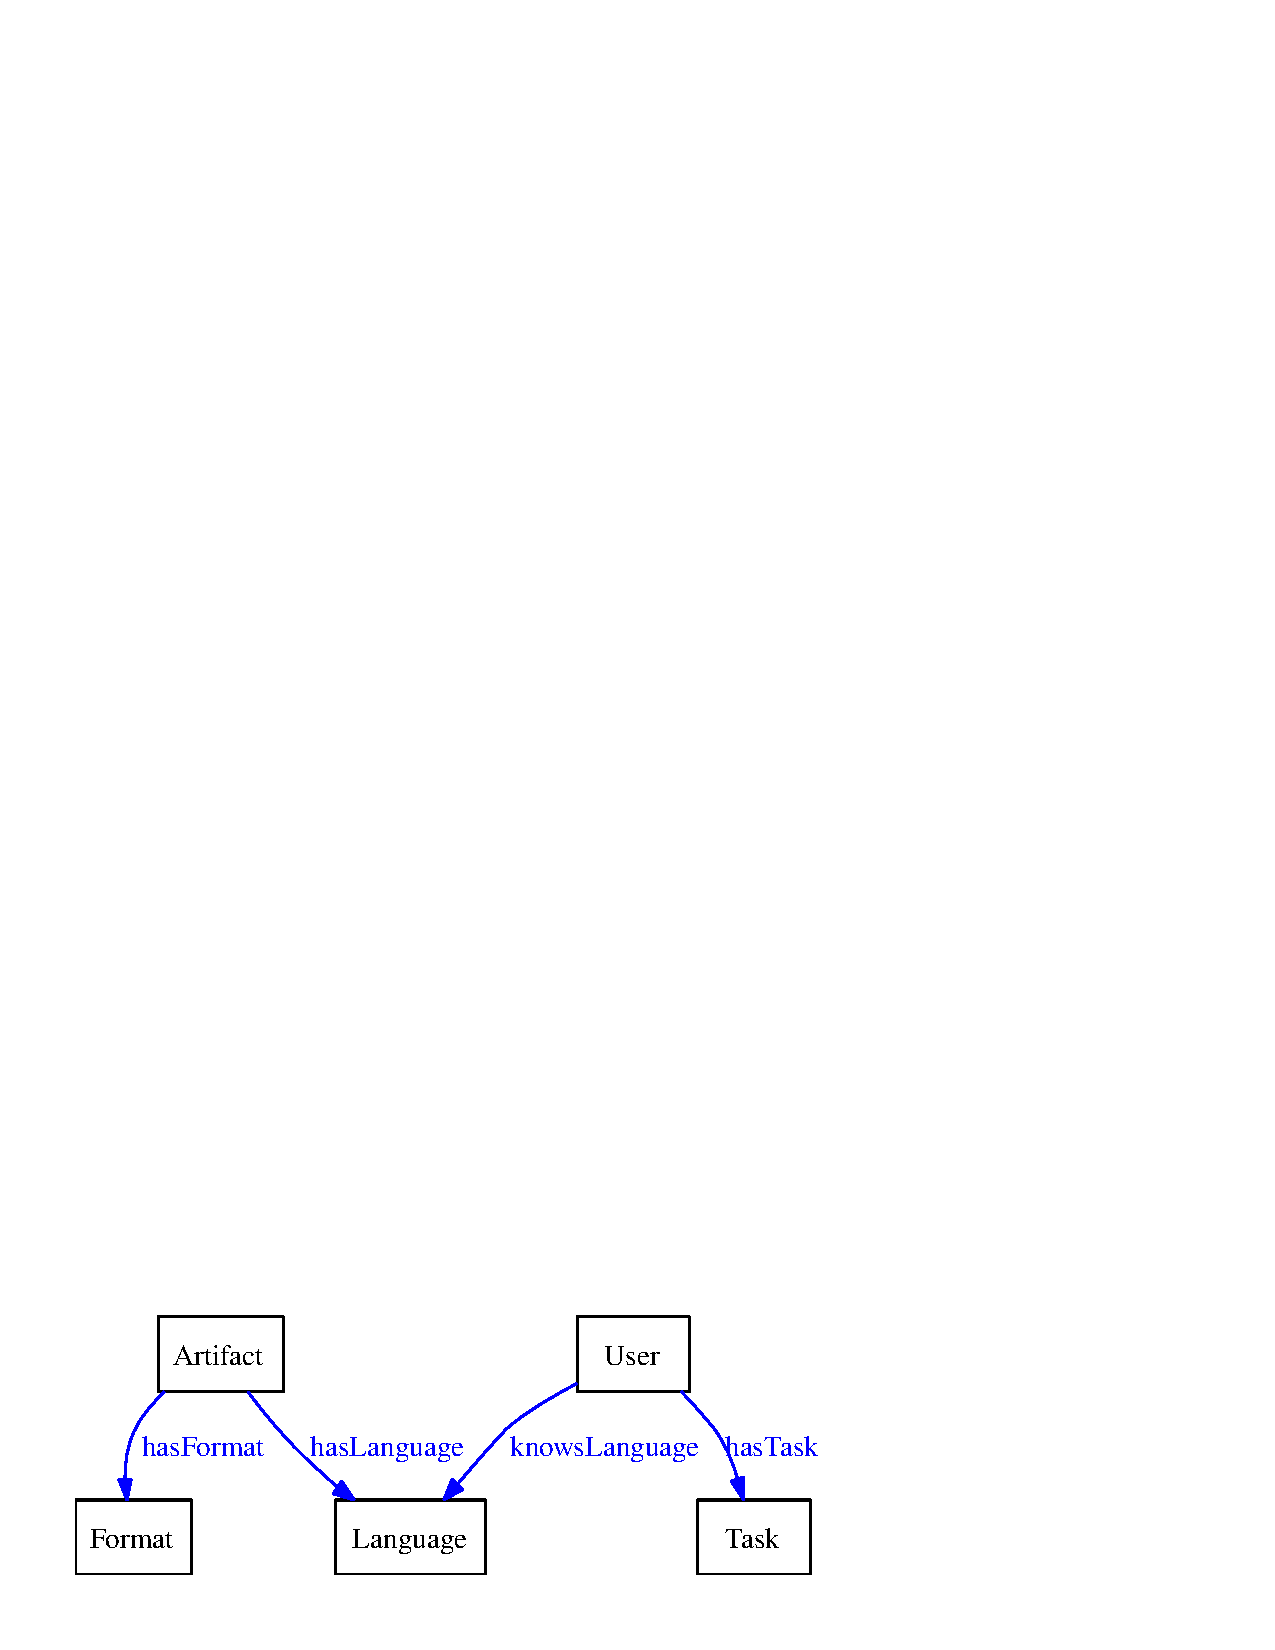
\includegraphics[width=0.5\textwidth]{pictures/centralfive.pdf}
  \caption{The five central concepts of the common upper ontology}
  \label{fig:centralFive}
\end{figure}


\begin{table}[htb]
\centering\small\sffamily
\begin{tabular}{p{0.13\textwidth}@{\hspace*{4mm}}p{0.55\textwidth}@{\hspace*{4mm}}p{0.22\textwidth}}
  \toprule
  \textbf{Concept}&\textbf{Description} &\textbf{Example/sub-concept} \\
  \midrule
  Artifact &The artifact is the central parent concept for all
    kinds of objects like documents, source files, compiled files,
    programs, NLP services, parameters, and annotations. Each field of
    application will most likely introduce its own artifacts.&
    Document, Tool, Parameter\\

   & & \\
  
  Format &Every artifact must have a format. For our language
    service infrastructure, it is important to know what formats the
    input and output of a service have in order to handle them
    correctly. &PDF, HTML\\

   & & \\
  
  User & In order to respond to a user's context, we also have to
    have some knowledge on the user himself. Which 
    languages does he know? What is he working on? & EnglishLearner\\

   & & \\
  
   Language & Languages are orthogonal to formats. Just as it is
   important to know if a file is binary or text, it is important to
   know if it is a Java source file or a manual written in HTML, or
   an article written in Spanish. NLP services are often language
   specific.& English, French, Java\\

   & & \\
  
   Task & Tasks further connect users and services. A task expresses
   a user's goal. If we know that goal, and we know what each of our
   offered services are good for, we can  match the two pieces of
   information and, ideally, provide the user with services that are
   useful to him. & TranslationTask\\
   \bottomrule
\end{tabular}
\caption{The five central concepts of the upper ontology}
\label{tab:top5}
\end{table}

Note that, while artifacts must have a format, they are not required
to have a language. Format information helps us to differentiate
between various kinds of artifacts, e.g., it enables us to tell a GATE
annotation from an executable program. We consider this kind of
information essential and relatively easy to provide -- even if there
is no obvious format, or the format is uncertain, we can most likely
still rely on generic formats like ``plain text file'' or ``binary
file''. On the other hand, it is not always intuitive to give a
language for a given artifact. E.g., we would hesitate to say that a
GATE annotation specifying a part of speech has a certain language.
Likewise, it is not very intuitive to say that a runtime parameter has
a language. Due to these difficulties, we leave the language as an
optional attribute for artifacts.

\paragraph{More Concrete Artifacts.} \emph{Tools}, like an NLP tool,
are a subconcept of \emph{artifacts}. A tool possibly processes
artifacts as input and can produce artifacts as output. These are
modeled with the \emph{consumesInput} and \emph{producesOutput}
relations in our ontology. Moreover, we mentioned parameters that a
tool can have, which is modeled by the \emph{hasParameter}
relation. For our domain, \emph{documents} are of great importance, in
particular natural language documents. These documents all have
languages (English, French, Java, etc.), modeled by the
\emph{hasLanguage} relation. As natural language documents are very
common and important, we introduce a sub-concept of \emph{Document}
called \emph{NaturalLanguageDocument}, which has a
\emph{hasNaturalLanguage} property.

In order to work with documents, they often must somehow be identified
and retrieved. In fact, the \sa server must be able to pull documents
for analysis from the Internet.  Thus, when we model such an input
document in our ontology, we must have a way to specify its URI
(Uniform Resource Identifier) by which we can address it. As not only
documents, but also other artifacts like Web services have to be
uniquely identified and addressed, we introduce \emph{hasIdentifier}
as an optional property for artifacts.  We define
\emph{IdentifiableArtifact} as a class whose members are artifacts and
have this property. In practice, the identifier can, and often will,
be a URI, but it does not have to be. For example, if we have a set of
elements with unique names, a simple string can be enough. With
\emph{hasIdentifier}, we provide an important property on the highest
level, while leaving the exact semantics to the concrete ontologies
and the applications that use them.

\paragraph{Output Modelling.} We introduced one more concept that is
not as obvious as the concepts introduced so far. Suppose there is an
NLP system that can, among others, output XML and OWL files. We would
model artifacts representing these file types, and create the
according \emph{producesOutput} relation pairs. However, which one of
the output variants is produced most likely depends on the way the
NLP system is invoked. Therefore, we have to somewhere store the
information, under which \emph{circumstances} a certain output is
produced. We could store it directly with the individual representing
the output. However, we feel that this information concerns more the
relationship between the system and the output, not the output
itself. Thus, we introduced a concept called \emph{IOArtifact} where
information on input and output relationships can be stored. We will
see a more concrete use of this concept in the following section, when
we concretize the upper ontology. By means of an
\emph{isActualArtifact} relation, we have \emph{IOArtifact}
individuals ``point'' to \emph{Artifact} individuals. They can be seen
as a proxy for artifacts.

We can see the artifact class, its sub-classes, and important
relations between these classes in Figure~\ref{fig:artifact}. A
textual overview is given in Table~\ref{tab:artifact}.
 
\begin{figure*}[htb]
  \centering
  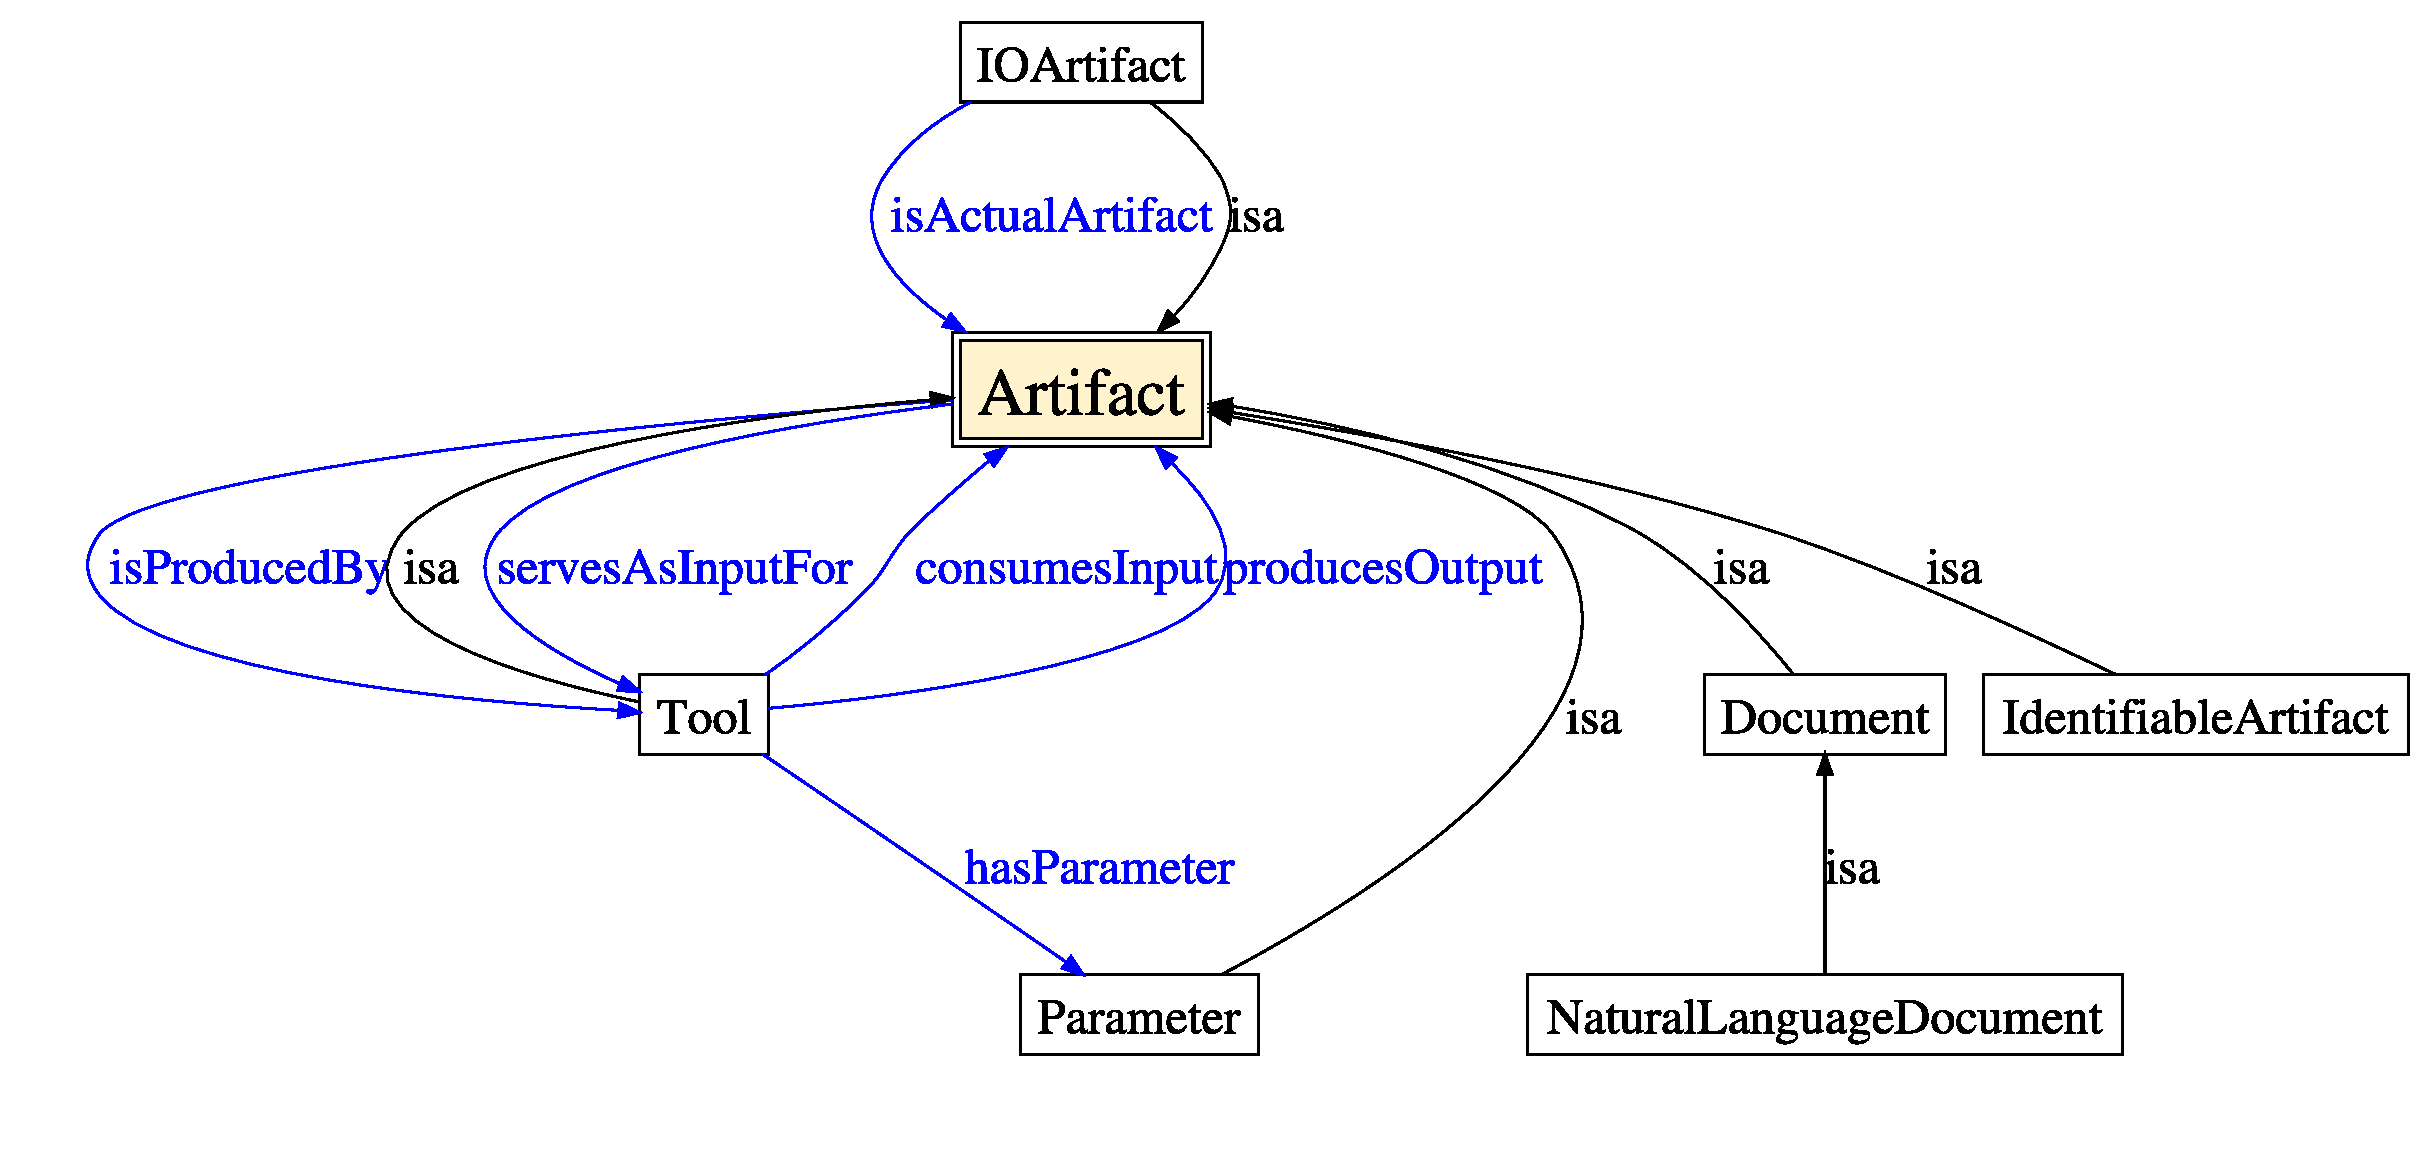
\includegraphics[width=1.0\textwidth]{pictures/artifact.pdf}
  \caption{The artifact base class with its subclasses}
  \label{fig:artifact}
\end{figure*}



We have not yet mentioned the relations \emph{servesAsInputFor} and
\emph{isProducedBy}. They are the inverse relations of
\emph{consumesInput} and \emph{producesOutput}, respectively, and have
been defined for reasons of completeness.



\begin{table}[tb]
\centering\small\sffamily
\begin{tabular}{p{0.20\textwidth}@{\hspace*{4mm}}p{0.42\textwidth}@{\hspace*{4mm}}p{0.28\textwidth}}
  \toprule 
  \textbf{Concept}&\textbf{Description} &\textbf{Example} \\
  \midrule

  Tool & Parent concept for all processing artifacts. Typically
  consumes some input and/or produces some output. & Single Document
  Summarizer, POS tagger \\

   & & \\

  Document & Artifact with a language (mandatory) & Web document,
  Java source code file \\

   & & \\

  Natural & Document with a & English Manual, \\
  Language Document & \emph{hasNaturalLanguage} property & French Novel \\

   & & \\

  Identifiable & Artifact that has some identifiable & Web document, GATE \\
  Artifact & string, e.g., a URI & processing pipeline \\

   & & \\

  Parameter & Parameter for a tool, typically with some type
  information  & Output format, desired summary length \\

   & & \\

  IOArtifact & Proxy for an input or output artifact, holding
  additional information on the relationship between the artifact and
  the consuming/producing tool  & Plain text output proxy, HTML output
  proxy \\

  \bottomrule
\end{tabular}
\caption{Sub-concepts of the \emph{Artifact} concept}
\label{tab:artifact}
\end{table}




\subsection{Specializing the Upper Ontology}
\label{sec:lsont}
The upper ontology that we have just introduced gives us several
things we need: artifacts, users, parameters, tools, etc. However, we
still lack some important NLP-specific concepts, which is why, in this
section, we substantiate the abstract upper ontology and refine it
into an ontology for language services. In particular, we include
concepts specific for the NLP subsystem in use by the \sa
architecture, GATE. Integrating a different NLP subsystem, like UIMA,
would require an alternative specialization focusing on UIMA specific
concepts and their relations.

\paragraph{New Tools and Artifacts.} We can now add a core concept for
the \sa architecture, NLP services. They are modeled as child concepts
to the \emph{Tool} concept, classifying language services in two
categories: \emph{IRTool} and \emph{NLPTool}. The semantics that we
want to convey by this separation is that an information retrieval
tool (\emph{IRTool}) finds documents, but leaves them untouched, while
an NLP tool processes documents and typically generates some new
artifact(s) from them. For NLP tools, input and output natural
languages can be specified. However, they do not have to be specified,
as there are also language-independent language services. Therefore,
if no input language is specified, we will assume that the language
service can handle any input language. Likewise, if no output language
is specified, we will assume that it can handle any output language.

Additionally to \emph{IRTool} and \emph{NLPTool}, we have one more
child concept named \emph{GATEPipeline}. While the two first concepts
imply certain semantics, the latter is defined solely via its
\emph{Format}, which has to be a certain GATE pipeline format. The
semantics of a \emph{GATEPipeline} are defined by its also being an
instance of one of the other two concepts. This means that a
\emph{GATEPipeline} can be an \emph{NLPTool} or an \emph{IRTool}.

The \emph{GATEPipeline} concept is obviously GATE specific: A sequence
of processing components is called \emph{pipeline} in GATE. In this
ontology, we do not model these processing components explicitly, as
an end user is not interested in single components of language services,
but in language services as a whole. Instances of \emph{GATEPipeline}
are the language services we offer the user through our architecture.

Having covered the \emph{Tool} extensions of our concrete ontology,
let us have a look at the artifacts they are associated with. As
mentioned, we need a semantic description of several GATE data
structures. Accordingly, we introduce new concepts as children of the
\emph{Artifact} concept. \emph{GATECorpus} represents a collection of
documents, which typically serves as input for a language service.
\emph{GATEAnnotation} instances describe the information which
language services add to a document. Annotations are organized into
annotation sets, hence we provide \emph{GATEAnnotation} with an
attribute specifying to which annotation set a given instance belongs
to. GATE annotations can have features, which are, as presented in
Section~\ref{sec:response}, included in our response
messages. Therefore, \emph{GATEAnnotation} instances can have an
unlimited number of \emph{hasFeature} attributes, which are simple
strings. \emph{GATERuntimeParameter} models parameters that control
certain aspects of a GATE pipeline, and is introduced as a sub-concept
to the already existing \emph{Parameter} concept. Along with these
artifact types, we have to introduce according new formats (remember
that artifacts are required to have a format). These are defined under
the common parent concept of \emph{GATEFormat}, which is a child of
the \emph{Format} concept.

\paragraph{Conditional Output.} The output of a tool can vary
depending on the input or on parameters: Suppose there is a language
service that produces an index of its input documents, similar to the
ones found at the back of many books.  Suppose further that this
indexer has a parameter \emph{outputFormat}, which can be set to
\emph{plain text} or \emph{html}. Therefore, the NLP service is
modelled to have two different output artifacts, a plain text file and
an HTML file. However, with the parameter settings available, only one
of them is produced at any single invocation of the NLP service, and
our server should know which one. The solution to this is provided
through the \emph{IOArtifact} concept already introduced, or, more
specifically, through a sub-concept thereof named
\emph{GATE\_OutputArtifact}.  Instances of \emph{GATE\_OutputArtifact}
have a property \emph{necessaryParameterSetting}, thus connecting an
output artifact to a certain parameter value. This parameter value is
represented through an instance of a newly introduced concept called
\emph{ParameterValuePair}. Therefore, in the example of the indexer, the
plain text output file would be associated with a
\emph{ParameterValuePair} instance holding the right parameter value
for plain text output, and the HTML output file would be associated
with one holding the value for HTML output. The server would then
compare the parameter value sent by the client to these values, and
thus know which output can actually be expected.


\paragraph{Concepts and Relationships.} The most important
additional concepts and relations of the more concrete ontology are
shown in Figure~\ref{fig:artifact2}, and also listed in
Table~\ref{tab:newconcepts}. Concepts and relations that are already
present in the upper ontology are drawn more faintly, and some of them
have been omitted entirely to keep the diagram clearer.

\begin{figure*}[tb]
  \centering
  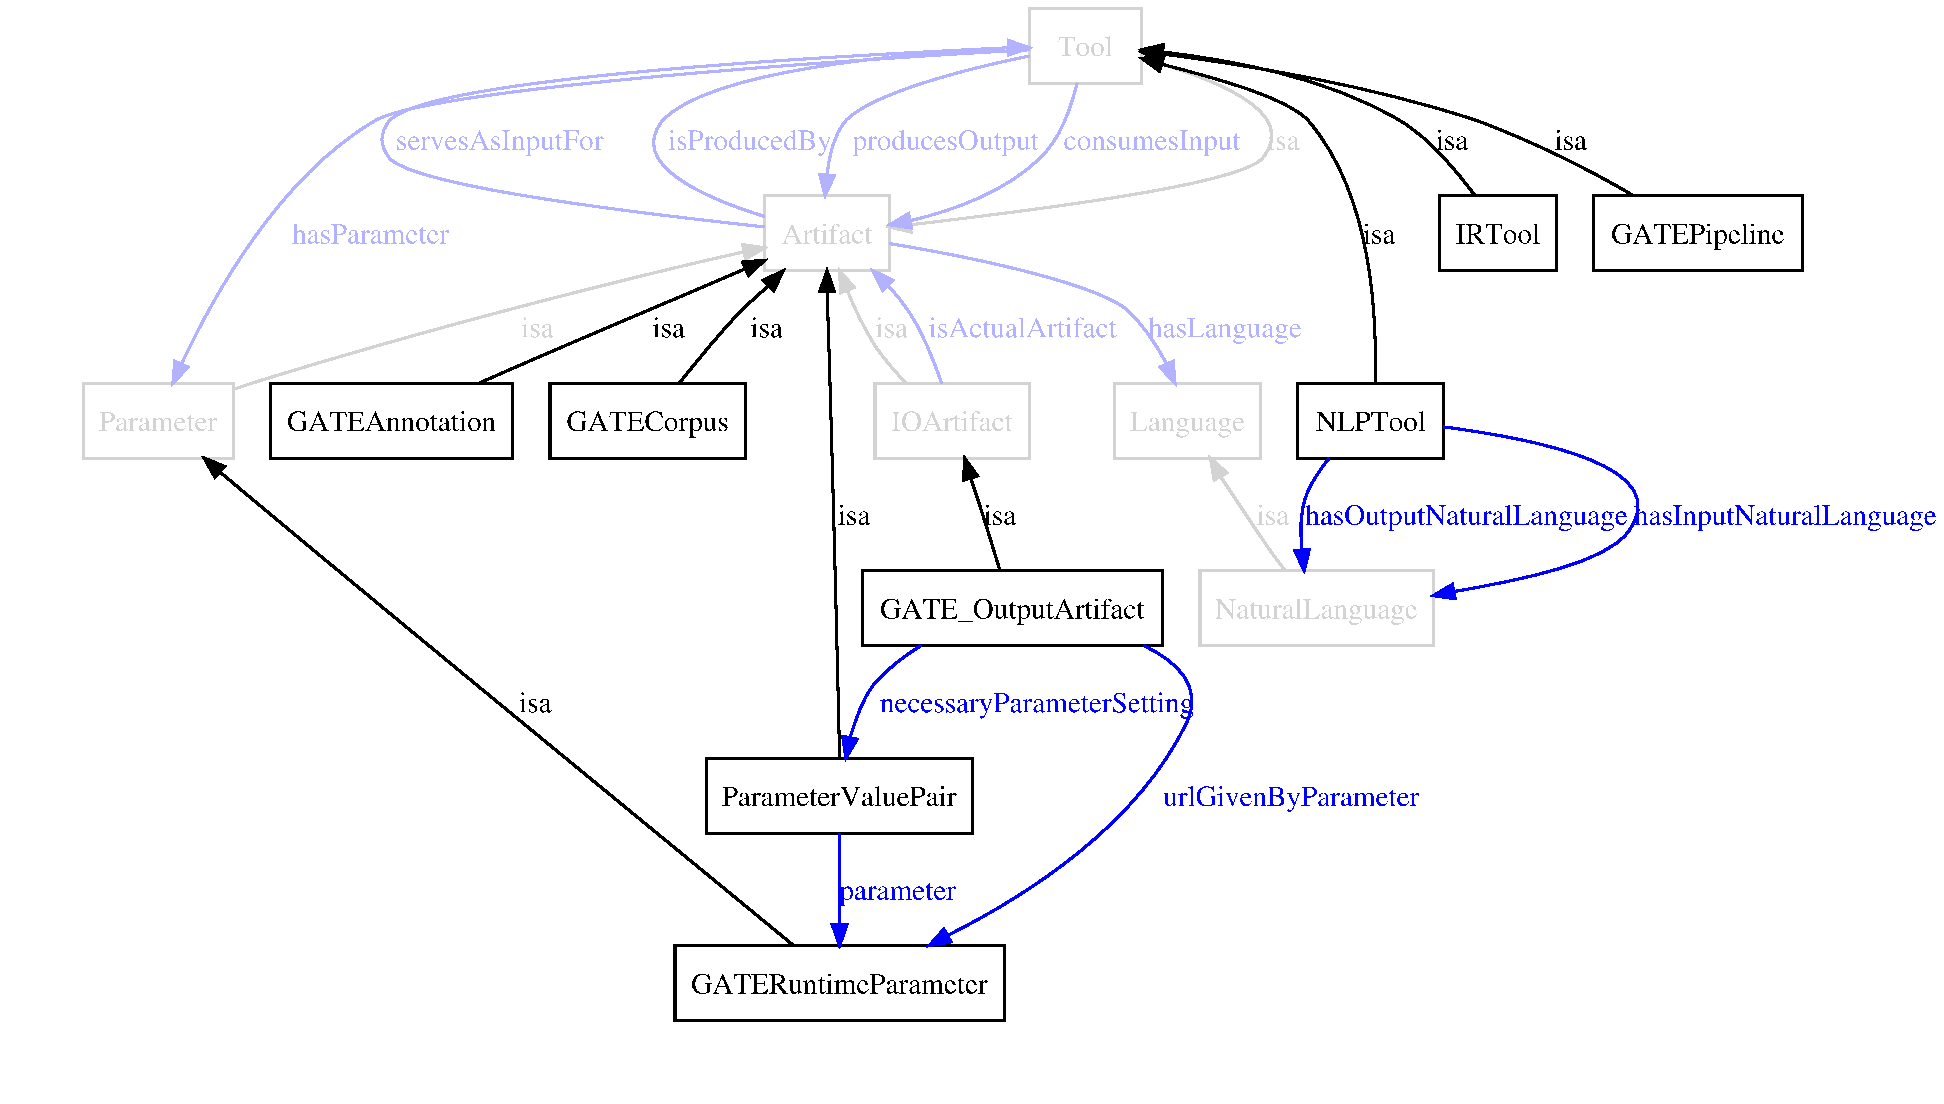
\includegraphics[width=1.0\textwidth]{pictures/artifact2.pdf}
  \caption{Additional classes introduced in the specialized ontology}
  \label{fig:artifact2}
\end{figure*}

\begin{table}[tb]
\centering\small\sffamily
\begin{tabular}{p{0.20\textwidth}@{\hspace*{4mm}}p{0.42\textwidth}@{\hspace*{4mm}}p{0.28\textwidth}}
  \toprule 
  \textbf{Concept}&\textbf{Description} &\textbf{Example} \\
  \midrule

  IRTool & Instances of this concept compile a collection of
  documents, usually in response to some query.  & \emph{YahooSearch}
  \\

   & & \\

  NLPTool & Instances of \emph{NLPTool} process or analyze documents,
  and usually produce new information from them. & \emph{Summarizer},
    \emph{Person Extractor} \\

   & & \\

  GATE Pipeline & The GATE specific implementation of a language
  service.  & \emph{Summarizer}, \emph{Person Extractor} \\

   & & \\

  GATE Annotation & GATE annotations represent linguistic and semantic
  information that has been added to a document. They can have
  \emph{hasFeature} attributes. & \emph{PersonAnnotation},
  \emph{LocationAnnotation}  \\

   & & \\

  GATE Corpus & A collection of documents, usually serving as input
  for a language service.  & \emph{StandardGATECorpus} \\

   & & \\

  GATE Runtime Parameter & Many language services accept parameters
  that influence their behaviour. Type, default value, and other
  information can be specified for a parameter.  &
  \emph{outputFileParameter}, \emph{summaryLengthParameter} \\

   & & \\

  GATE Output Artifact & Holds additional information on the
  relationship between a GATE pipeline and its possible output &
  \emph{HTMLOutputArtifact}, \emph{PlainTextOutputArtifact}  \\

   & & \\

  Parameter Value Pair & Can be used to specify certain values for a
  parameter. Usually used in combination with
  \emph{GATEOutputArtifact} and the \emph{necessaryParameterSetting}
  relation.  & \emph{htmlSetting}, \emph{plainTextSetting} \\
  \bottomrule
\end{tabular}
\caption{Concepts newly introduced in the concrete ontology for
  language services}
\label{tab:newconcepts}
\end{table}

The relation called \emph{urlGivenByParameter} connecting a GATE
output artifact to a GATE runtime parameter remains to be explained.
Often, when language services produce a file as output, they offer the
user an option to specify where this file should be stored. In our
architecture, our server has to take advantage of this so that it can
take the file and pass it on to the requesting client. The
\emph{urlGivenByParameter} relation informs the server which parameter
it can set to specify the desired output destination of an output
file.


\begin{table}[tb]
\centering\small\sffamily
\begin{tabular}{p{0.20\textwidth}@{\hspace*{2mm}}p{0.15\textwidth}@{\hspace*{2mm}}p{0.15\textwidth}@{\hspace*{2mm}}p{0.40\textwidth}}
  \toprule 
  \textbf{Property Name}&\textbf{Domain} &\textbf{Range} &\textbf{Description} \\
  \midrule

  consumesInput & Tool & Artifact & Lists the GATERuntimeParamter(s) of a language service
  \\

   & & \\

  hasFormat & Artifact & Format & Specifies the format of a language service (GATEPipeline\_Format)
  \\

   & & \\

  hasParameter & Tool & Parameter & Lists the GATERuntimeParamter of a language service
  \\

   & & \\

  producesOutput & Tool & Artifact & Specifies the output of a language service (e.g. GATEOutput\_Artifact)
  \\

   & & \\

  \bottomrule
\end{tabular}
\caption{Object Properties for Artifact}
\label{tab:newconcepts}
\end{table}


\begin{table}[tb]
\centering\small\sffamily
\begin{tabular}{p{0.20\textwidth}@{\hspace*{4mm}}p{0.15\textwidth}@{\hspace*{2mm}}p{0.15\textwidth}@{\hspace*{2mm}}p{0.40\textwidth}}
  \toprule 
  \textbf{Property Name}&\textbf{Domain} &\textbf{Range} &\textbf{Description} \\
  \midrule

  hasLabel & Artifact & xsd:string & Specifies the label to be shown to clients
  \\

   & & \\

  appFileName & GATEPipeline & xsd:string & The actual filename of the GATE application, without path, e.g. Durm-Indexer
  \\

   & & \\

  hasGateName & Artifact & unset & Specifies the name of the Artifact.
  \\

   & & \\

  mergeInputDocuments & Artifact & xsd:boolean & Specifies if input documents are to be merged into one before they are passed to this language service
  \\

   & & \\

  publishAsNLPService & Tool & xsd:boolean & Specifies if an NLP tool should be published to client(s)
  \\

   & & \\

  \bottomrule
\end{tabular}
\caption{Datatype Properties for Artifact}
\label{tab:newconcepts}
\end{table}




\begin{table}[tb]
\centering\small\sffamily
\begin{tabular}{p{0.20\textwidth}@{\hspace*{2mm}}p{0.15\textwidth}@{\hspace*{2mm}}p{0.15\textwidth}@{\hspace*{2mm}}p{0.40\textwidth}}
  \toprule 
  \textbf{Property Name}&\textbf{Domain} &\textbf{Range} &\textbf{Description} \\
  \midrule

  hasFormat & Artifact & Format & Specifies the format of a language service (Standard\_GATEAnnotation\_Format)
  \\

   & & \\  

  \bottomrule
\end{tabular}
\caption{Object Properties for GATEAnnotation}
\label{tab:newconcepts}
\end{table}


\begin{table}[tb]
\centering\small\sffamily
\begin{tabular}{p{0.20\textwidth}@{\hspace*{4mm}}p{0.15\textwidth}@{\hspace*{2mm}}p{0.15\textwidth}@{\hspace*{2mm}}p{0.40\textwidth}}
  \toprule 
  \textbf{Property Name}&\textbf{Domain} &\textbf{Range} &\textbf{Description} \\
  \midrule

  hasFeature & GATEAnnotation & xsd:String & Specifies the additional features of an annotation
  \\

   & & \\

  hasGATEName & Artifact & xsd:String & The name of the Annotation
  \\

   & & \\  

  \bottomrule
\end{tabular}
\caption{Datatype Properties for GATEAnnotation}
\label{tab:newconcepts}
\end{table}



\begin{table}[tb]
\centering\small\sffamily
\begin{tabular}{p{0.20\textwidth}@{\hspace*{2mm}}p{0.15\textwidth}@{\hspace*{2mm}}p{0.15\textwidth}@{\hspace*{2mm}}p{0.40\textwidth}}
  \toprule 
  \textbf{Property Name}&\textbf{Domain} &\textbf{Range} &\textbf{Description} \\
  \midrule

  hasFormat & Artifact & Format & Specifies the format of a language service (Standard\_GATEAnnotation\_Format)
  \\

   & & \\

  isActualArtifact & IOArtifact & Artifact & Specifies the actual GATEAnnotaiton Individual
  \\

   & & \\

  isProducedBy & Artifact & Tool & The Artifact that prodcues the output (e.g. GATE pipeline)
  \\

   & & \\  

  \bottomrule
\end{tabular}
\caption{Object Properties for GATEOutputArtifact}
\label{tab:newconcepts}
\end{table}


\begin{table}[tb]
\centering\small\sffamily
\begin{tabular}{p{0.15\textwidth}@{\hspace*{4mm}}p{0.20\textwidth}@{\hspace*{2mm}}p{0.15\textwidth}@{\hspace*{2mm}}p{0.40\textwidth}}
  \toprule 
  \textbf{Property Name}&\textbf{Domain} &\textbf{Range} &\textbf{Description} \\
  \midrule
  
  hasGATEName & Artifact & xsd:string & The name of the GATEOutputArtifact
  \\

   & & \\  

  isPerDocument & GATE\_OutputArtifact & xsd:boolean & Specifies is this artifact produced for each input document, or is it valid for a whole input corpus.
  \\

   & & \\ 
  \bottomrule
\end{tabular}
\caption{Datatype Properties for GATEOutputArtifact}
\label{tab:newconcepts}
\end{table}



\begin{table}[tb]
\centering\small\sffamily
\begin{tabular}{p{0.20\textwidth}@{\hspace*{2mm}}p{0.15\textwidth}@{\hspace*{2mm}}p{0.15\textwidth}@{\hspace*{2mm}}p{0.40\textwidth}}
  \toprule 
  \textbf{Property Name}&\textbf{Domain} &\textbf{Range} &\textbf{Description} \\
  \midrule

  hasFormat & Artifact & Format & Specifies the format of a language service (Standard\_GATE\_RTP\_Format)
  \\

   & & \\

  servesAsInputFor & Artifact & Tool & Specifies the tool (e.g. pipeline) that the parameter serves as input for.
  \\

   & & \\
  
  \bottomrule
\end{tabular}
\caption{Object Properties for GATERuntimeParameter}
\label{tab:newconcepts}
\end{table}


\begin{table}[tb]
\centering\small\sffamily
\begin{tabular}{p{0.12\textwidth}@{\hspace*{4mm}}p{0.25\textwidth}@{\hspace*{2mm}}p{0.20\textwidth}@{\hspace*{2mm}}p{0.40\textwidth}}
  \toprule 
  \textbf{Property Name}&\textbf{Domain} &\textbf{Range} &\textbf{Description} \\
  \midrule
 
  hasLabel & Artifact & xsd:string & Specifies the label to be shown to clients
  \\

   & & \\


  isOptional & IOArtifact or Parameter & xsd:boolean & Specifies if the runtime parameter for the processing resource is optional.
  \\

   & & \\ 
  
  defaultValue & GATERuntimeParameter & xsd:string & The name of the GATEOutputArtifact
  \\

   & & \\  

  hasGATEName & Artifact & xsd:string & The name of the GATERuntimeParameter
  \\

   & & \\ 

  paramType & GATERuntimeParameter & owl:oneOf\{``string'' ``double'' ``int'' ``boolean'' ``url'' ``list(string)'' ``list(double)'' ``list(int)'' ``list(boolean)'' ``list(url)''\} & Specifies The type of a parameter. Use string, double, int, or boolean for now.
  \\

   & & \\ 

  prName & GATERuntimeParameter & xsd:string & Specifies the name of the processing resource the parameter belongs to.
  \\

   & & \\ 
  \bottomrule
\end{tabular}
\caption{Datatype Properties for GATERuntimeParameter}
\label{tab:newconcepts}
\end{table}


We have noted that GATE pipelines contain several processing
resources, each of which can, in theory, take parameters. Obviously,
the parameter values sent by the client must be assigned correctly,
i.e., to the correct processing resources. To satisfy this
requirement, \emph{GATERuntimeParameter} instances hold an attribute
called \emph{prName}, the ``pr'' standing for ``processing
resource''. Additionally, parameters hold a \emph{paramType} and a
\emph{defaultValue} attribute.


\paragraph{Concatenation of Language Services.}
Language services can also be concatenated. In order to do this, we
introduced an attribute to the \emph{GATEPipeline} concept, called
\emph{concatenationOfPipelines}. If a language service is actually a
concatenation of several GATE pipelines. This attribute holds a
comma-separated list of the according pipeline names. We chose this
flat data type approach over object relations because it is an easier
way of guaranteeing the correct order of the language services. OWL
does not support ordering in an obvious way, and although a design
pattern for modelling sequences exists, % \cite{owlseq},
we felt that our simple approach was sufficient for the situation at
hand.


\subsubsection{Querying the \sa Ontology}
The ontology described so far now contains the information
needed to dynamically find, load, parametrize, and execute available
language services, based on user's current task and language
capabilities.  In our implementation, it is queried using Jena's
SPARQL\footnote{SPARQL Query Language for RDF, see
  \url{http://www.w3.org/TR/rdf-sparql-query/}} interface, using the
context information delivered by the client plug-in, in order to
recommend applicable Semantic Assistants.

For example, when a recommendation request is received, with a context
object saying the user knows English and German, the generated SPARQL
query should restrict the available services to those that deliver
English or German as output language. A simplified version of such a
generated query is shown below:

\begin{lstlisting}[language=SQL,xleftmargin=8mm,columns=flexible]
SELECT ?x ?name
WHERE { ?x sa:hasGATEName ?name  .
         {?x cu:hasFormat sa:GATECorpusPipeline_Format}  . {
             {?x sa:hasOutputNaturalLanguage cu:en}  UNION 
                 {?x sa:hasOutputNaturalLanguage cu:de}}
}
\end{lstlisting}
Once the SPARQL query has been generated, it is passed to the
\texttt{OntModel} instance containing the language service
descriptions. The results are then retrieved from this object,
converted into the corresponding client-side versions, and returned to
the client.


\section{Service Invocation and Result Passing}
In this section, we provide details on the communication between the
clients and the server in the \sa architecture.

\subsection{Service Invocation}
\label{sec:invoc}
Clients must be able to pass a single document as well as multiple
documents as input to an NLP service. The \sa architecture allows to
pass documents either literally or via a URI. In order to implement
these requirements while maintaining a uniform way of service
invocation, a client must pass two lists to the server: The first list
contains one URI per document passed to the language service.  Thus,
the number of URI entries in this list equals the number of documents
passed. If a document is passed via URI, then its URI entry in the
first list is simply its URI. If the document is to be passed
literally, we put a special URI that is not a URL in the first list,
which acts as a signal. In that case, the second list comes into
play. The second list contains one entry for each document that is
passed literally, and each entry is the document text itself. Thus,
when the server encounters a URL in the first list, it can use this
URL to access the document and when a special URI is given, the server
advances to the next entry in the second list and finds the document
contents there. Obviously, order is important when we use this
algorithm. The use of the two lists is illustrated in
Figure~\ref{fig:twolists}, where four input documents are passed. The
first and the fourth document are passed via URL, while the second and
the third are passed literally.

\begin{figure}
  \centering
  %\vspace*{-9mm}
  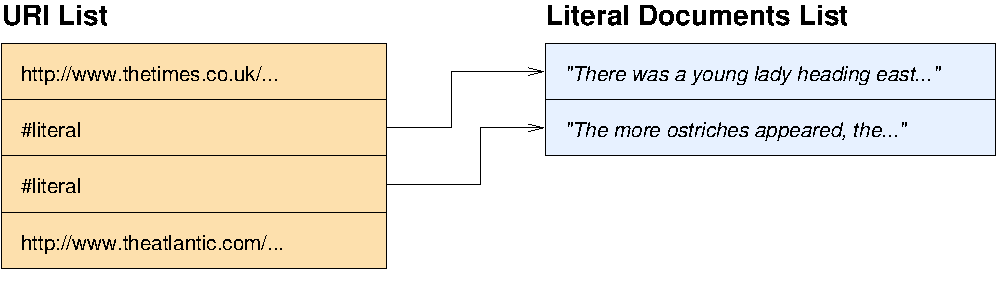
\includegraphics[width=0.8\textwidth]{pictures/twolists}
  \vspace*{-0.4cm}
  \caption{The two lists representing the input documents for an NLP service}  
  \label{fig:twolists}
\end{figure}

Besides the name and the input for a language service, we might need
the client to provide a list of parameters. Therefore, a list of
parameters as described in the previous section is passed along. The
\emph{Value} field of a parameter holds the user-specified value this
parameter should be assigned. Finally, we enable the communication of
user context by passing a representation thereof, as introduced in the
previous section. Table~\ref{tab:invocation} lists all the data
elements transmitted on language service invocation.

\begin{table}
 \centering\small\sffamily
 \begin{tabular}{p{0.22\textwidth}@{\hspace*{4mm}}p{0.45\textwidth}@{\hspace*{4mm}}p{0.2\textwidth}}
   \toprule
   \textbf{Field} & \textbf{Meaning} & \textbf{Example} \\
   \midrule
   NLP service name & The unique identifier of the desired & \emph{English Single} \\
    & language service & \emph{Document Summarizer} \\

    & & \\

   URI list & A list of actual input document URIs and special URIs
   signalling that this document is passed literally. Every input
   document is represented here. & See Fig.~\ref{fig:twolists}  \\

    & & \\

   Document text list & List of document texts, only of those
   documents that are passed literally & See Fig.~\ref{fig:twolists}
   \\

    & & \\

   Parameter list & Transports the parameter values that the client
   specifies & See Table~\ref{tab:param} \\

    & & \\

   User context & The user context, as specified in &
   \emph{[userLangs=en,fr} \\
    & Section~\ref{sec:contextservice} & \emph{docLang=en]}\\
 
   \bottomrule
\end{tabular}
 \caption{Data fields sent from the client when invoking an NLP service}
 \label{tab:invocation}
\end{table}

While language services can most likely be invoked without the current
user context at hand, knowing some facts can prove useful before or
after the invocation. Thus, the invocation could be cancelled if it
is detected that the chosen language service does not fit the input
document(s), or one could tailor the generated output to the user
client's preferences or capabilities.


\subsection{Language Service Results}
\label{sec:response}
Once a language service has finished its work, we want to collect its
results and pass them, in an appropriate format, on to the client. The
\sa architecture allows for different result formats (document
annotation, new documents, results files such as ontologies) and
passes them in a uniform XML response format back to the client.

The basic structure of our response message is rather simple. No
matter what the contents of a message are, they are always be enclosed
in a single \texttt{saResponse} element, the ``sa'' standing for
``Semantic Assistant''. Within this enclosing element, the results
produced by the language service are listed one by one. In
Figure~\ref{list:response1}, this is illustrated for a language
service which produces two different results. Here, they are called
\emph{result1} and \emph{result2}. In reality, they might be an
annotation and a file, or two different annotations, etc.

\begin{figure}[htb]
\begin{lstlisting}[language=XML,xleftmargin=8mm,columns=flexible]
<?xml version="1.0"?>
<saResponse>
    <result1>
        ...
    </result1>
    <result2>
        ...
    </result2>
</saResponse>
\end{lstlisting}
\vspace*{-2mm}
\caption{Schematic structure of an example response with two results}
\label{list:response1}
\end{figure}


\paragraph{Result from GATE Annotations.} With the outer structure of a response
message in place, we have to properly define how specific results are
represented. We take care of annotations first, especially annotations
in GATE (see the GATE documentation for a description of the GATE
document data model if you do not know about document annotations).
Instead of \texttt{result1} or \texttt{result2} in the example above,
we will thus have \texttt{annotation} tags. An important aspect of an
annotation obviously is its name, or type, e.g., \emph{Protein} or
\emph{Person}.  Additionally, for GATE annotations, we include the
annotation set that the annotation is contained in. Thus, we have an
\texttt{annotation} element with \texttt{type} and
\texttt{annotationSet} attributes.

There might be several input document to an NLP service, and an
annotation is always associated with a specific document. Therefore, the
response first lists all input documents within each
\texttt{annotation} tag, using \texttt{document} tags. If the URL of a
document is known, it is included in the corresponding \texttt{document}
tag. However, if a document has been passed literally, we do not have
a URL, so we cannot include it in the response message either. This
seems to be a problem when several documents are passed literally: How
does the client know which result belongs to which document? However,
the order of the documents is maintained as it was when the client
sent them as input.  Therefore, the client is able to correctly assign
the results to the input documents.

For every document, we then list the occurrences of the annotation in
question, using \texttt{annotationInstance} elements. Instances hold a
\texttt{start} and an \texttt{end} attribute, which are character
offsets and which enable the client to locate the instance in the
input text. Moreover, there is a \texttt{content} attribute, which
holds the text located between the \texttt{start} and \texttt{end}
text positions. Finally, annotations can hold an arbitrary number of
so-called features. Features that the system integrator thinks could
be of interest are listed as child elements of the
\texttt{annotationInstance} elements. We can see an example output
with three different annotations (\emph{Date}, \emph{Person}, and
\emph{Location}) and one document in Figure~\ref{list:response2}. The
\emph{Person} and \emph{Location} annotations each have one feature
listed -- \emph{gender} in the case of the person, \emph{locType} in
the case of the location. The document has been passed via URL, which
is why this URL is also included in the response.

\begin{figure}[htb]
\begin{lstlisting}[language=XML,xleftmargin=8mm,columns=flexible]
<?xml version="1.0"?>
<saResponse>
  <annotation type="Date" annotationSet="">
    <document url="http://www.thetimes.co.uk/...">
      <annotationInstance content="yesterday" start="76" end="85">
      </annotationInstance>
      <annotationInstance content="today" start="1056" end="1061">
      </annotationInstance>
      <annotationInstance content="past ten years" start="6477" end="6491">
      </annotationInstance>
    </document>
  </annotation>
  <annotation type="Person" annotationSet="">
    <document url="http://www.thetimes.co.uk/...">
      <annotationInstance content="Tony Blair" start="65"  end="75">
        <feature name="gender" value="male" />
      </annotationInstance>
      <annotationInstance content="Rupert Murdoch" start="2357" end="2371">
        <feature name="gender" value="male" />
      </annotationInstance>
      <annotationInstance content="Mr Blair" start="3133"  end="3141">
        <feature name="gender" value="male" />
      </annotationInstance>
    </document>
  </annotation>
  <annotation type="Location"  annotationSet=""  >
    <document url="http://www.thetimes.co.uk/...">
      <annotationInstance content="Iraq" start="1510" end="1514">
        <feature name="locType" value="country" />
      </annotationInstance>
      <annotationInstance content="Downing Street" start="4576" end="4590">
        <feature name="locType" value="" />
      </annotationInstance>
    </document>
  </annotation>
</saResponse>
\end{lstlisting}
\vspace*{-2mm}
\caption{Result example with three annotations and their detected instances}
\label{list:response2}
\end{figure}


\paragraph{Result Files.} NLP services can also generate new files as
a result -- these can be of any format, depending on the concrete
components deployed in the pipeline. Instead of embedding the file
itself (which can be quite large) directly into the response, we only
pass an identifier for the file, along with some format information.
The client can evaluate this information, and, if it decides to do so,
request the result file itself by using the identifier sent to it. The
server then sends the actual file. Again, we have an example response
in Figure~\ref{list:response3}. The \texttt{outputFile} element holds
format information, both in form of a MIME type string and a human
readable one. The identifier for the result file is given through the
\texttt{url} attribute which refers to the server's file system.

\begin{figure}
\begin{lstlisting}[language=XML,xleftmargin=8mm,columns=flexible]
<?xml version="1.0"?>
<saResponse>
  <outputFile url="file:/tmp/serviceResult-..."
              mimeType="text/html" format="HTML Document" />
</saResponse>
\end{lstlisting}
\vspace*{-2mm}
\caption{Result example with one resulting HTML file}
\label{list:response3}
\end{figure}


\paragraph{Formal Response Message Format Definition.} The complete
response format definition DTD can be found in
Figure~\ref{list:dtd}. It defines documents of the type
\texttt{saResponse}. The \texttt{saResponse} element can contain
arbitrarily many \texttt{annotation} elements and \texttt{outputFile}
elements. Annotations, annotation instances, features, and output
files are defined accordingly.

\begin{figure}
\begin{lstlisting}[language=XML,xleftmargin=8mm,columns=flexible]
<!DOCTYPE saResponse [

  <!ELEMENT saResponse ( annotation*, outputFile* ) >

  <!ELEMENT annotation ( document+ ) >
  <!ATTLIST annotation annotationSet CDATA #IMPLIED >
  <!ATTLIST annotation type NMTOKENS #REQUIRED >

  <!ELEMENT annotationInstance ( feature* ) >
  <!ATTLIST annotationInstance content CDATA   #REQUIRED >
  <!ATTLIST annotationInstance end     NMTOKEN #REQUIRED >
  <!ATTLIST annotationInstance start   NMTOKEN #REQUIRED >

  <!ELEMENT document ( annotationInstance* ) >
  <!ATTLIST document url CDATA #IMPLIED >

  <!ELEMENT feature EMPTY >
  <!ATTLIST feature name  NMTOKEN #REQUIRED >
  <!ATTLIST feature value CDATA   #REQUIRED >

  <!ELEMENT outputFile EMPTY >
  <!ATTLIST outputFile format   CDATA #REQUIRED >
  <!ATTLIST outputFile mimeType CDATA #REQUIRED >
  <!ATTLIST outputFile url      CDATA #REQUIRED >

]>
\end{lstlisting}
\vspace*{-2mm}
\caption{The document type definition (DTD) for our response messages}
\label{list:dtd}
\end{figure}

We have now discussed the most important data exchange processes. In
the next section, we want to ask the question where this data on NLP
services comes from, and how it is organized.

\section{Developing a New Client for the Semantic Assistants Architecture}
We have now covered the most important and interesting implementation
issues, and are ready, with the knowledge we have, to give
step-by-step instructions to connect a client application to our
architecture, and thus to the functionality of NLP services. These
instructions depend a bit on the client implementation language. As we
described earlier, our implementation of the client-side abstraction
layer consists of Java classes packaged in a single Java archive
(\texttt{.jar}) file. Hence, if the client application is able to make
use of Java archives, connecting to our architecture is done as
follows:

\begin{enumerate}
\item Have your application import the Java archive containing the
    implementation of the client-side abstraction layer (CSAL).

\item If necessary, tell the CSAL the address of the Web service
    endpoint. The CSAL classes that need to know the address have a
    default value for it.

\item Create a \texttt{SemanticServiceBrokerService} object, which
    serves as a factory for proxy objects.

\item Create such a proxy object. This is your ``remote control'' to
    the Web service. You can call all methods that have been published
    through the Web service on this object.
\end{enumerate}

After these four steps, a Java-enabled client application can get
lists of available language services as well as invoke these language
services. A code example, where an application obtains such a proxy
object and invokes the \texttt{getAvailableServices} method on it to
find available language analysis services, is shown below:

\begin{lstlisting}[language=Java,xleftmargin=4mm,columns=flexible]
// Create a factory object
SemanticServiceBrokerService service = new SemanticServiceBrokerService();
// Get a proxy object, which locally represents the service endpoint (= port)
SemanticServiceBroker broker = service.getSemanticServiceBrokerPort();
// Proxy object is ready to use. Get a list of available language services.
ServiceInfoForClientArray sia = broker.getAvailableServices();
\end{lstlisting}

A client application developer who cannot use the Java archive that
implements the CSAL still has access to the WSDL description of our
Web services. If there are automatic client code generation tools
available for the programming language of his choice, the developer
can use these to create CSAL-like code, which can then be integrated
into or imported by his application. In this case, the integration
steps would be similar to the steps enumerated above, with the
additional step of generating client-side code from the WSDL
description before the first step.

If there are no such code generation tools, the client application has
to implement the communication with the server itself. To do this, it
must create the SOAP messages that represent method invocations, and
send them to the Web service endpoint. Also, it must receive the
response messages from the server, and extract the relevant
information in them. Usually, however, there are standard libraries
that facilitate these tasks.



% \subsection{Control Flow Overview}
% \begin{figure}[htb]
%   \centering
%   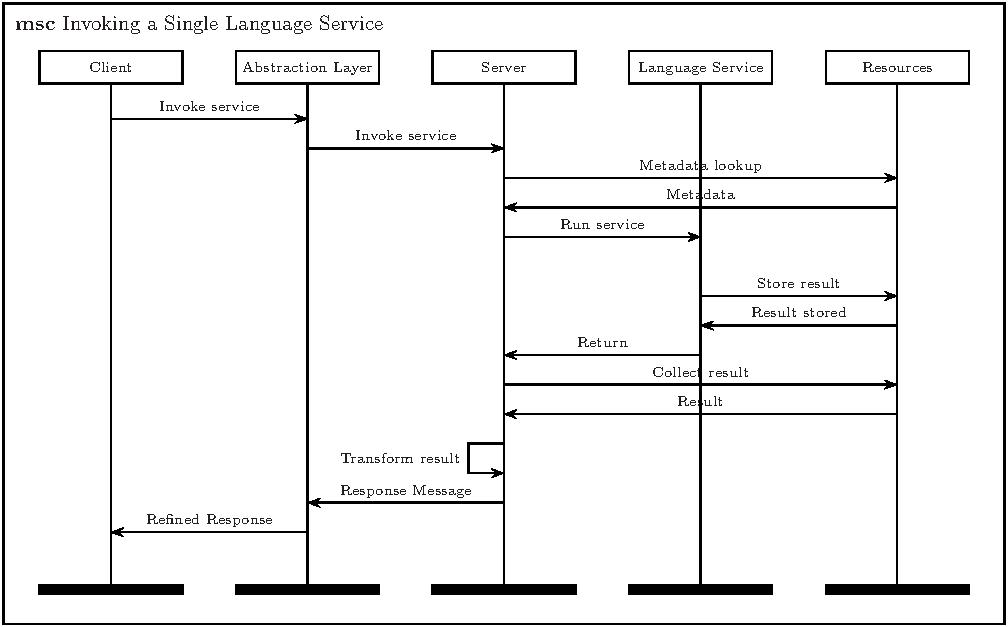
\includegraphics[width=0.5\textwidth]{pictures/seqInvoke1.pdf}
%   \caption{The client invokes a language service and receives a
%     result}
%   \label{fig:seqInvoke1}
% \end{figure}
% Once requested, the language service is executed asynchronously by our
% architecture, allowing the user to continue his work (he can even
% execute additional services).  The sequence diagram in
% Figure~\ref{fig:seqInvoke1} shows the execution of a service
% through the various tiers described in Section~\ref{sec:implementation} Note
% that all low-level details of handling language services, such as
% metadata lookup, parametrization, and result handling, are hidden from
% the client plug-in through our client-side abstraction layer.
